% !TEX root = ../../../main.tex
% 来源：中学数学实验教材·第一册（代数）
% 章节：有理数系 / 有理数系的基本性质
% 原始文件：1.tex，行 3245-3253
% 类型：tikz
% ---
		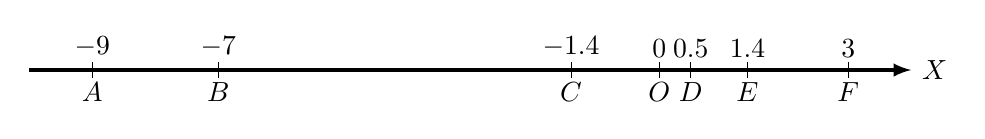
\begin{tikzpicture}[xscale=.8,>=latex]
		
		\draw[->, very thick] (-10,0)--(4,0)node[right]{$X$};        
		
		\foreach \x/\y in {-9/A,-7/B,-1.4/C,0/O,0.5/D, 1.4/E,3/F}
		{
			\draw (\x,-.1)node[above=4pt]{$\x$}--(\x,.1)node[below=4pt]{$\y$};
		}
		\end{tikzpicture}
